Tras haber expuesto las motivaciones y el contexto en el que se engloba este Trabajo de Fin de Grado, en este capítulo daremos una explicación más detallada del problema que se
intenta resolver.


\section{Descripción del problema}
\label{sec:descripcion del problema}
El propósito general es la mejora de la herramienta Scratch4Robots, que traduce programas en el lenguaje visual Scratch a programas en Python dentro del entorno ROS o del entorno JdeRobot. Como principales subobjetivos tenemos:
\begin{itemize}
\item \textbf{Mejora de la herramienta Scratch4Robots}:

Esta mejora la llevamos a cabo en la agregación de nuevos bloques visuales, y la refactorización de los ya existentes para aumentar las posibilidades y facilitar la usabilidad de la herramienta. Además buscamos acercar al usuario la herramienta con una documentación ajustada a usuarios con perfiles poco técnicos, acompañado de ejemplos didácticos.

\item \textbf{Generación de paquete ROS, para
facilitar su uso}:

Se va a publicar la herramienta en forma de paquete ROS, de forma que pueda ser instalable en cualquier máquina con un sistema operativo Ubuntu, y pueda acceder a sus funcionalidades a través de la consola de comandos, sin necesidad de descargar el código fuente de la herramienta. De esta forma evitamos que el usuario tenga que indagar en nuestro código fuente para tener que ejecutar nuestro nodo.

\item \textbf{Validación experimental con robots simulados}:

Buscamos exponer con forma de ejemplos prácticos, posibles casos de uso de la herramienta, de distintas complejidades.
\end{itemize}


\section{Requisitos}
\label{sec:requisitos}

Para cumplir los objetivos marcados de forma satisfactoria, debemos además satisfacer
los siguientes requisitos:

\begin{itemize}
\item El desarrollo deberá ser autocontenido en lo que sea posible, esto quiere decir que todas las librerías y dependencias de nuestra herramienta deberán estar contenidas en su interior. La programación se realizará en el
lenguaje Python.
\item El software desarrollado deberá ser compatible con Ubuntu 16.04, ROS-kinetic y Scratch 2.0 serán los únicos elementos indispensables para el correcto funcionamiento de nuestra herramienta.
\item Todos los componentes desarrollados deberán ser compatibles tanto trabajando en entornos simulados, como usando robots reales, esto se consigue usando todas las abstracciones de las que nos provee JdeRobot, y de todas las funcionalidades del middleware ROS.
\end{itemize}



\section{Metodología de trabajo}
\label{sec:metodologia}

Dada la naturaleza del proyecto, y al igual que en cualquier otro proyecto de software, es necesario el uso de un modelo que defina el ciclo de vida de la aplicación. Para el desarrollo de este proyecto hemos decidido adoptar el modelo de desarrollo en espiral.\\

El modelo en espiral consiste en una serie de ciclos que se repiten en forma de
bucle, cada ciclo representa un conjunto de actividades. Las actividades no están
prefijadas \textit{a priori}, sino que se eligen en función de las realizadas previamente. Estos ciclos se irán ejecutando hasta que la aplicación sea aceptada y no requiera otro
ciclo. Este modelo, definido por Barry Boehm en 1986, se basa en una espiral en la que cada iteración representa un conjunto de actividades.Estas actividades no tienen prioridad, se elegirá en la fase de análisis de riesgos. Así, cada iteración está dividida en las siguientes actividades:

\begin{itemize}
\item Determinar objetivos: en esta actividad se definirá el objetivo de la iteración actual. Siguiendo este modelo el objetivo final del proyecto se divide en subobjetivos, los cuales hemos definido anteriormente.
\item Análisis de riesgo: en esta actividad, se lleva a cabo varios estudios con el propósito de conocer las posibles amenazas o eventos no deseados que se puedan producir en el objetivo actual.
\item Desarrollar y probar: llegados a este punto será necesario la verificación del correcto funcionamiento realizado en la iteración para subsanar los errores y que estos no prosigan en las siguientes iteraciones. En este caso después de cada nuevo desarrollo se pasaba una batería de pruebas funcionales que aseguraban el funcionamiento de nuestra herramienta tras los nuevos desarrollos.
\item Planificación: en esta actividad se revisarán las fases anteriores para determinar si se debería continuar. En las reuniones semanales con el tutor se establecía la planificación y alcance de las siguientes actividades.
\end{itemize}

\begin{figure}[h]
    \centering
    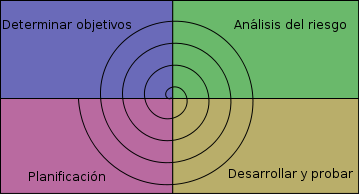
\includegraphics[width=0.75\textwidth]{img/metodologia_espiral}
    \caption{Desarrollo en espiral}
    \label{fig:espira}
\end{figure}

Para materializar estas actividades e iteraciones mantuvimos reuniones semanales con el tutor durante todo el desarrollo del trabajo. De este modo, cada semana marcábamos un nuevo subobjetivo. Si el anterior se había completado, planificábamos el siguiente. Si por el contrario, no sé había completado, ahondábamos en el objetivo actual para corregir los errores o volver a planificarlo.\\

Todo el código fuente generado se mantuvo en un repositorio Git\footnote{\url{https://github.com/JdeRobot/Scratch4Robots}}. De este modo el tutor y cualquier otra persona interesada tiene acceso en cualquier momento al código, además nos apoyamos del sistema de apertura de \textit{issues} en el repositorio remoto Git para cada implementación que se necesitaba desarrollar para la mejora del proyecto. De esta forma queda documentado todo el proceso de desarrollo de la herramienta.\\

Durante todo el desarrollo del trabajo se realiza un seguimiento de los objetivos a cumplimentar a través de una bitácora de trabajo\footnote{\url{http://jderobot.org/Scarrion-tfg}}.

\section{Plan de trabajo}
\label{sec:plan}

Simplificaremos la labor a desarrollar en este Trabajo de Fin de Grado en varios puntos:
\begin{itemize}
\item \textbf{Familiarización con el entorno software}: 

Como punto de partida, y durante el comienzo del trabajo nos centramos en la familiarización con el software que vamos a utilizar y desarrollar en un futuro. Estudamos JdeRobot, que es la plataforma de desarrollo principal utilizada en la mayoría de proyectos realizados en el departamento de robótica de la URJC. El objetivo principal de esta fase es aprender a utilizar este software, sus componentes y sus drivers para más adelante utilizarlos como parte de nuestro proyecto. Como parte del aprendizaje, se desarrolla una herramienta externa al core principal pero que usa de librerías y recursos de ella.\\

Además de JdeRobot, posteriormente nos centramos en ROS, que está muy presente en este trabajo, necesitando un conocimiento en profundidad de su arquitectura, su uso y de los componentes necesarios para desarrollar nuestro paquete propio basado en ROS.
\item \textbf{Estudio de Kurt y otras bibliotecas implicadas en la herramienta}: 

En un segundo periodo estudiaremos las bibliotecas implicadas en el funcionamiento interno de la herramienta, como punto fuerte de esta fase está el estudio de la biblioteca Kurt, que nos permite obtener toda la información necesaria de un proyecto Scratch, conocimiento de su API y su funcionamiento interno para saber qué podemos llegar a obtener y como usar esa información para proporcionar una traducción robusta al lenguaje Python.
\item \textbf{Mejora y desarrollo de nuevas funcionalidades}: 

Una vez entendido el software del que nos ayudamos para el desarrollo de la herramienta, es momento comenzar con la implementación de las mejoras. Aumentando el número de bloques robóticos propios que podremos usar en Scratch, esto es desarrollar la lógica detrás de cada bloque, todo programado en Python y la integración de estos bloques con Scratch. Dividimos los bloques entre bloques de uso genéricos, bloques aptos para drones y robots con ruedas. Estos bloques deben tener una funcionalidad muy específica y funcionar en armonía con el resto, tanto los propios de la aplicación Scratch como los nuevos bloques generados por nosotros propios de aplicaciones robóticas.
\item \textbf{Integración y documentación}: 

Una vez terminadas las mejoras de funcionalidades de la herramienta, nos centraremos en la mejora de su integración y uso.

Como objetivo tenemos la creación y publicación de nuestra herramienta como un paquete ROS, fácilmente instalable y ejecutable en cualquier entorno Ubuntu.

Con la documentación buscamos hacer la herramienta lo más intuitiva posible, mejorando scripts de lanzamiento y de generación de código. Creando ejemplos autocontenidos para una rápida demostración de la potencia de la herramienta y generando tutoriales tanto escritos como con vídeo para evitar confusiones.
\item \textbf{Validación Experimental}:

Por último buscamos la validación del funcionamiento de la herramienta, desarrollando ejemplos de distintas complejidades.
\end{itemize}
